%----------------------------------------------------------------------------------------
%	TITLE PAGE
%----------------------------------------------------------------------------------------

\begingroup
\thispagestyle{empty}
\AddToShipoutPicture*{\put(0,0){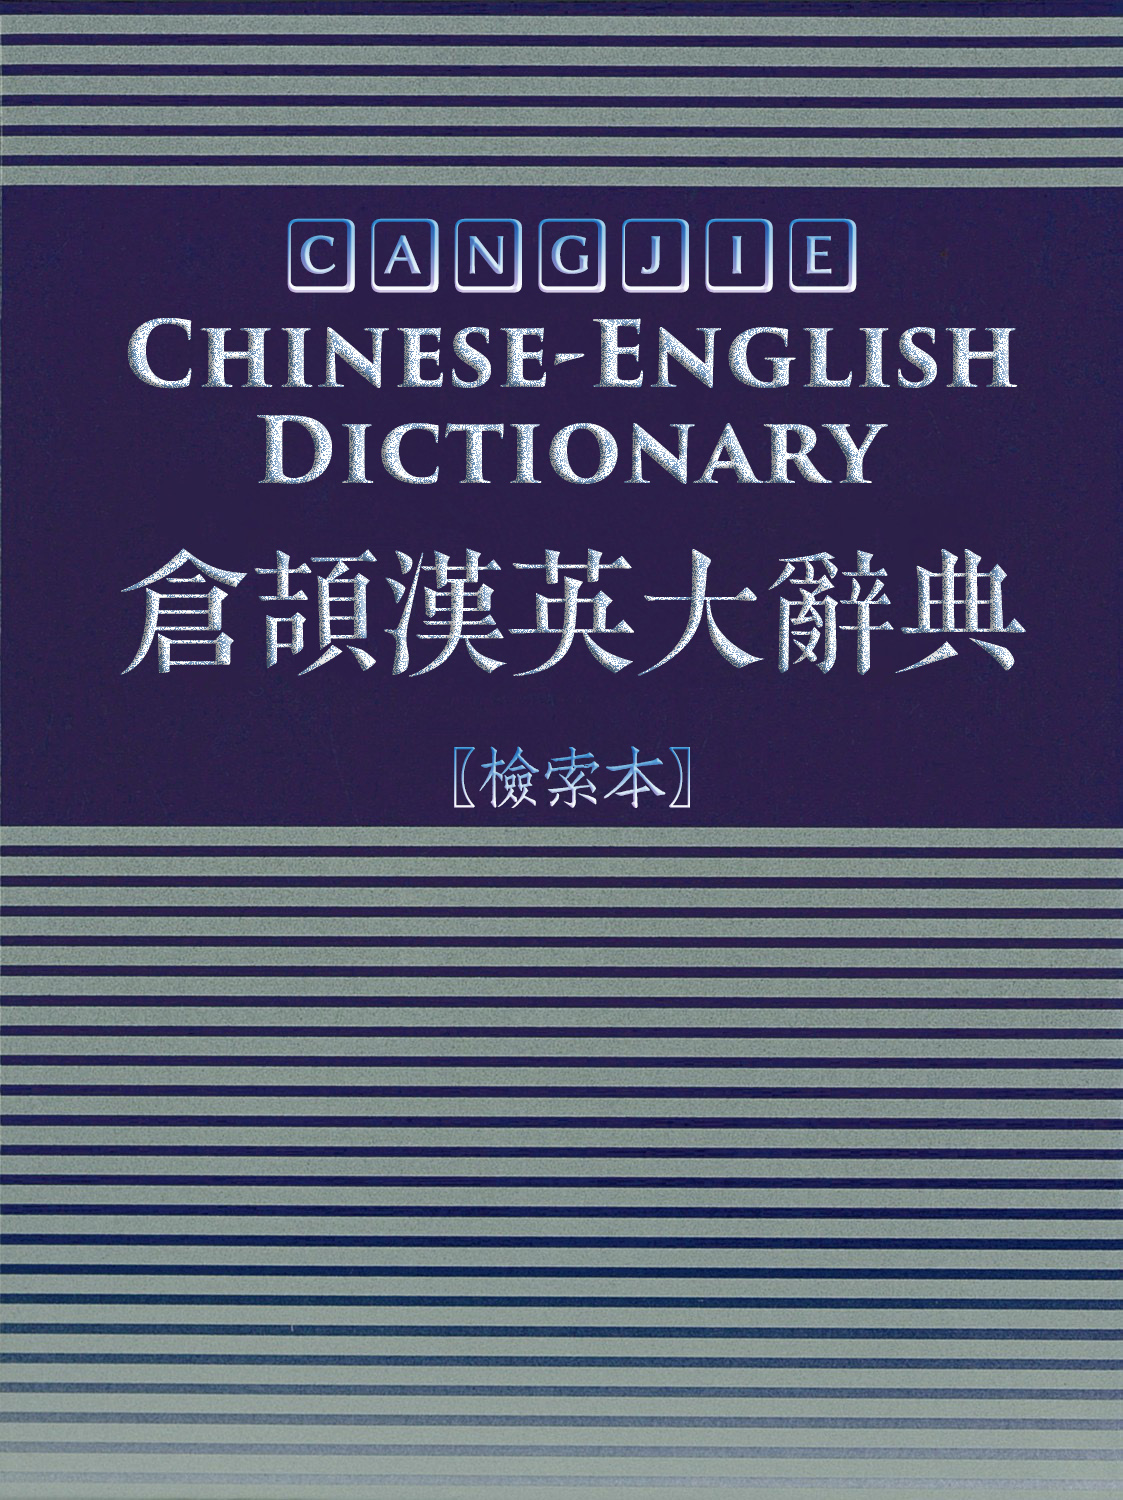
\includegraphics[width=\paperwidth,height=\paperheight]{title.jpg}}} % Image background
\vspace*{9cm}
\endgroup
\newpage

\begingroup
\thispagestyle{empty}
\AddToShipoutPicture*{\put(0,0){
\includegraphics[width=\paperwidth,height=\paperheight]{background.pdf}}} % Image background
\centering
\begin{tikzpicture}[remember picture,overlay]
\node (rect) at (6,-11.7) [minimum width=27cm,minimum height=8.8cm,line width=4pt,rounded corners=10pt,draw=myred,fill=black,fill opacity=0.5] {};
\pgftext[center,x=7.7cm,y=-8.8cm]{{\fontsizec{.81cm}\color{white}\tpfontb Marc Meng}};
\pgftext[center,x=7.7cm,y=-11.2cm]{{\fontsizec{2.2cm}\color{white}\ZSKS 倉頡漢英辭典}};
\pgftext[center,x=7.7cm,y=-13.5cm]{{\fontsizec{.6cm}\color{white}\tpfontb Cangjie Chinese-English Dictionary}};
\end{tikzpicture}
\endgroup

%----------------------------------------------------------------------------------------
%	COPYRIGHT PAGE
%----------------------------------------------------------------------------------------

\newpage
~\vfill
\thispagestyle{empty}

\noindent {\profonta Cangjie Chinese-English Dictionary} by {\profontc Marc Meng}\\

\noindent {\unifonti Copyleft \textcopyleft ~~2006–2016 Marc Meng} \\ % Copyright notice

\noindent {\profonte Marcm Press}\\ % Publisher

\noindent ISBN: 1-292-02482-8

\noindent \url{https://github.com/elegist/Cangjie-Chinese-English-Dictionary}\\ % URL

	\noindent
	{\unifont Developed with \TeX{}Live 2014. Composed and typeset with \XeLaTeX\ v.\ \the\XeTeXversion{}\XeTeXrevision{}, Memoir class v.\ 3.6j (patch 6.0f), hyperref v.\ 6.83c, fontspec v.\ 2.2b.  First printing, October 2014}

%----------------------------------------------------------------------------------------
